\chapter{Implementation}\label{chapter:implementation}
\section{Plugin}
iBSched is implemented as an extension to SLURM in the form of a scheduler plugin. A Slurm plugin is a dynamically linked code object which is loaded explicitly at run time by the Slurm libraries. A plugin provides a customized implementation of a well-defined API connected to tasks such as authentication, interconnect fabric, and task scheduling. There are several other existing scheduler plugins of SLURM such as: the default(FCFS) plugin, Backfill, wiki and wiki2(Interfaces to external schedulers) etc. A related plugin that is of importance to scheduling is the priority plugin because the job queue is first constructed and then sorted based on priorities before the scheduling algorithm runs through it. Slurm provides a basic priroity plugin and a multifactor priority plugin. The basic version provides a standard FIFO based job priority whereas the multifactor version provides priorities to job based on several factors such as age, fair-share, job size(also considers the job duration to calculate a weight factor for job size relative to time), partition, quality of service etc. The multifactor priority plugin has been refactored for this work to be better suitable for our implementation. Specifically, the multifactor priority plugin now assigns priority to jobs based on age and size(also considers the job duration to calculate a weight factor for job size relative to time). As its default behavior it also re-calculates periodically the priority of the jobs.\\ \\
%%%%%
For the current scope of the work, iRTSched has been implemented as an independent binary that talks to iBSched via the negotiation protocol. The purpose of this independent binary is to fake an actual runtime scheduler by simulating the runtime states of the system in time by employing the runtime scheduling algorithm and also negotiating with iBSched. In reality, a full-fledged runtime scheduler will be managing the resources in the invasic partition, will launch the jobs and perform dynamic resource management. In order to evaluate the negotiation-based separation of batch and runtime scheduling system, a simulation of the same involving a fake runtime scheduler would be very useful and sufficient for our objectives. 
\section{Data Structures}
This section will enumerate some of the important data structures that are a part of the implementation.\\ \\
\textbf{Job Mappings}
\begin{lstlisting}[mathescape]
enum job_hint {
        COMP_BOUND,
        MEMORY_BOUND,
        IO_BOUND,
	NONE
};

enum job_type {
        RIGID,
        MOLDABLE,
        EVOLVING,
        MALLEABLE
};

typedef struct qos_rsrc {   
        uint32_t min;
        uint32_t max;
} qos_rsrc_t;
\end{lstlisting}
%%%%%%%%
\begin{lstlisting}[mathescape]
struct forward_job_details {
        qos_rsrc_t node_count;          /* Job resource requirements */
        uint16_t contiguous;            /* set if requires contiguous nodes */
        uint16_t cpus_per_task;         /* number of processors required for
                                         * each task */
        uint8_t hint;                   /* Job characteristic: IO / Compute / Memory bound */
        uint8_t job_type;                       /* Type of job: Static or Dynamic */
        uint32_t max_cpus;              /* maximum number of cpus */
        uint32_t min_cpus;              /* minimum number of cpus */

        /* job constraints: */
        uint32_t pn_min_cpus;           /* minimum processors per node */
        uint32_t pn_min_memory;         /* minimum memory per node (MB) OR
                                         * memory per allocated
                                         * CPU | MEM\_PER\_CPU */
        uint32_t pn_min_tmp_disk;       /* minimum tempdisk per node, MB */
        uint8_t share_res;              /* set if job can share resources with
                                         * other jobs */
        uint8_t whole_node;             /* 1: --exclusive * 2: --exclusive=user */
};
\end{lstlisting}
%%%%%%%
\begin{lstlisting}[mathescape]
struct forward_job_record {
        struct forward_job_details *details;    /* job details */
        uint32_t job_id;                /* job ID */
        uint32_t magic;                 /* magic cookie for data integrity */
        char *name;                     /* name of the job */
        bitstr_t *node_bitmap;          /* bitmap of nodes allocated to job */
        uint32_t node_cnt;              /* Current node count assigned */
        uint32_t min_nodes;
        uint32_t max_nodes;
        uint32_t priority;              /* relative priority of the job,
                                         * zero == held (don't initiate) */
        time_t start_time;              /* Expected or Actual start time */
        uint32_t time_limit;            /* time_limit minutes or INFINITE,
                                         * NO_VAL implies partition max_time */
        uint32_t time_min;              /* minimum time_limit minutes or
                                         * INFINITE,
                                         * zero implies same as time_limit */
};
\end{lstlisting}
%%%%%%%
\begin{lstlisting}[mathescape]
typedef struct request_resource_offer_msg {
        uint16_t value; /* info */
        List jobs2map; /* This is the list of jobs waiting to be dispatched. And communicates the current requirements to rt scheduler which 
                          can then try to suitably construct a resource offer to satisfy the requirements as best as possible */
} request_resource_offer_msg_t;
\end{lstlisting}
%%%%%%%%
\begin{lstlisting}[mathescape]
typedef struct resource_offer_resp_msg {
        uint16_t value;         /* info */
        List map_jobs2offer;    /* Jobs mapped to the given offer. This depends on whether the batch scheduler accepted / rejected / countered
                                 the resource offer it received */
        uint32_t error_code;    /* error code on failure */
        char   * error_msg;     /* error message on failure */
} resource_offer_resp_msg_t;
\end{lstlisting}
%%%%%%%
\textbf{Resource Offers}
\begin{lstlisting}[mathescape]
typedef struct job_resv {
        time_t end_time;        /* end time of reservation              */
        uint8_t full_nodes;        /* when reservation uses full nodes or not */
        uint32_t job_id;        /* job ID */
        bitstr_t *node_bitmap;  /* bitmap of reserved nodes             */
        uint32_t node_cnt;      /* count of nodes required              */
        time_t start_time;      /* start time of reservation            */
} job_resv_t;


typedef struct resource_offer_msg {
        uint16_t value;      /* info */
        uint8_t negotiation; /* if negotiation is ongoing then this value is 1 else it becomes 0 to indicate ischeduler that previous negotiat
                                ion is over */
        List resource_offer;   /* List of node space records */
        List resv_jobs;        /* List of jobs with actual reservations. Can also include jobs with virtual reservations that are those with
                                  future start / service times */
        uint32_t error_code;    /* error code on failure */
        char   * error_msg;     /* error message on failure */
} resource_offer_msg_t;
\end{lstlisting}
%%%%%%%%%%
\textbf{Feedback Reports}
\begin{lstlisting}[mathescape]
typedef struct job_status {
        uint32_t job_id;
        time_t run_time;
        time_t end_time;
        uint32_t node_cnt;
        bitstr_t *node_bitmap;
        uint32_t job_state;
} job_status_t;

typedef struct status_report_msg {
        List status_reports;
} status_report_msg_t;
\end{lstlisting}
%%%%%%%%%%%
\textbf{Running Job Record}
\begin{lstlisting}[mathescape]
struct run_job_record {
        uint32_t job_id;
        bitstr_t *node_bitmap;
        time_t start_time;
        uint32_t priority;
        uint32_t time_limit;
        uint8_t hint;
        uint8_t job_type;
        time_t end_time;
        time_t orig_end_time;
        uint32_t job_state;
        uint32_t orig_node_cnt;
        uint32_t node_cnt;
        uint32_t last_node_cnts[2];
        bitstr_t *next_node_bitmap;
        uint32_t next_node_cnt;
        uint32_t depend_job_id;
        uint32_t depend_job_prio;
        uint32_t save_depend_job_id;
        uint32_t save_depend_job_prio;
        uint32_t min_nodes;
        uint32_t max_nodes;
        uint8_t adapt;  /* 0 - No change, 1 - Expand, 2 - Shrink */
        uint8_t transformed;
        time_t exp_end_time;
        time_t last_resize_time;
        uint32_t adapt_interval;
};
\end{lstlisting}
%%%%%%%
\textbf{Node Space Map}
\begin{lstlisting}[mathescape]
typedef struct node_space_map {
        time_t begin_time;
        time_t end_time;
        bitstr_t *avail_bitmap;
        int next;       /* next record, by time, zero termination */
} node_space_map_t;
\end{lstlisting}
%%%%%%%%
\section{Important APIs}
For batch scheduler\\
\begin{lstlisting}[mathescape]
extern List schedule_invasic_jobs(resource_offer_msg_t *, List, uint16_t *, uint32_t *);

extern uint32_t adjustQoS_node_count(struct job_record *);

extern void resetQoS_node_counts();

extern int _decision_logic(List, int, uint32_t);

extern void *irm_agent(void *);

extern int receive_resource_offer(slurm_fd_t, slurm_msg_t *);

extern int process_resource_offer(resource_offer_msg_t *, uint16_t *, int *, List *, List);

extern int send_resource_offer_resp(slurm_msg_t *, char *, List);

extern int request_resource_offer(slurm_fd_t, List);

extern int _request_resource_offer(slurm_fd_t);  /* Wrapper for request_resource_offer to construct the list of job requirements to be sent */
\end{lstlisting}
%%%%%%%%%%%%%
For runtime scheduler\\
\begin{lstlisting}[mathescape]
extern int slurm_submit_resource_offer(slurm_fd_t, resource_offer_msg_t *, resource_offer_resp_msg_t **);

extern int wait_req_rsrc_offer (slurm_fd_t, request_resource_offer_msg_t **);

extern int process_rsrc_offer_resp(resource_offer_resp_msg_t *, int, resource_offer_msg_t **);

extern int compute_feedback(status_report_msg_t *);

extern int create_resource_offer(int, List, uint16_t, resource_offer_msg_t **);

extern bitstr_t * _try_transf(bool);

extern int _commit_state(bool);

extern bitstr_t * _restore_state(void);

extern int _update_job_states(void);

extern time_t next_job_endtime(void);

extern bool _get_delta(uint32_t *, time_t, time_t);

extern void _initialize_state(void);

extern int _decision_logic(resource_offer_msg_t *, List, int, bool);
\end{lstlisting}
%%%%%%%%%%%%%
\section{State Machine Diagrams}
\subsection{iBSched}
\begin{figure}[!t]
\centering
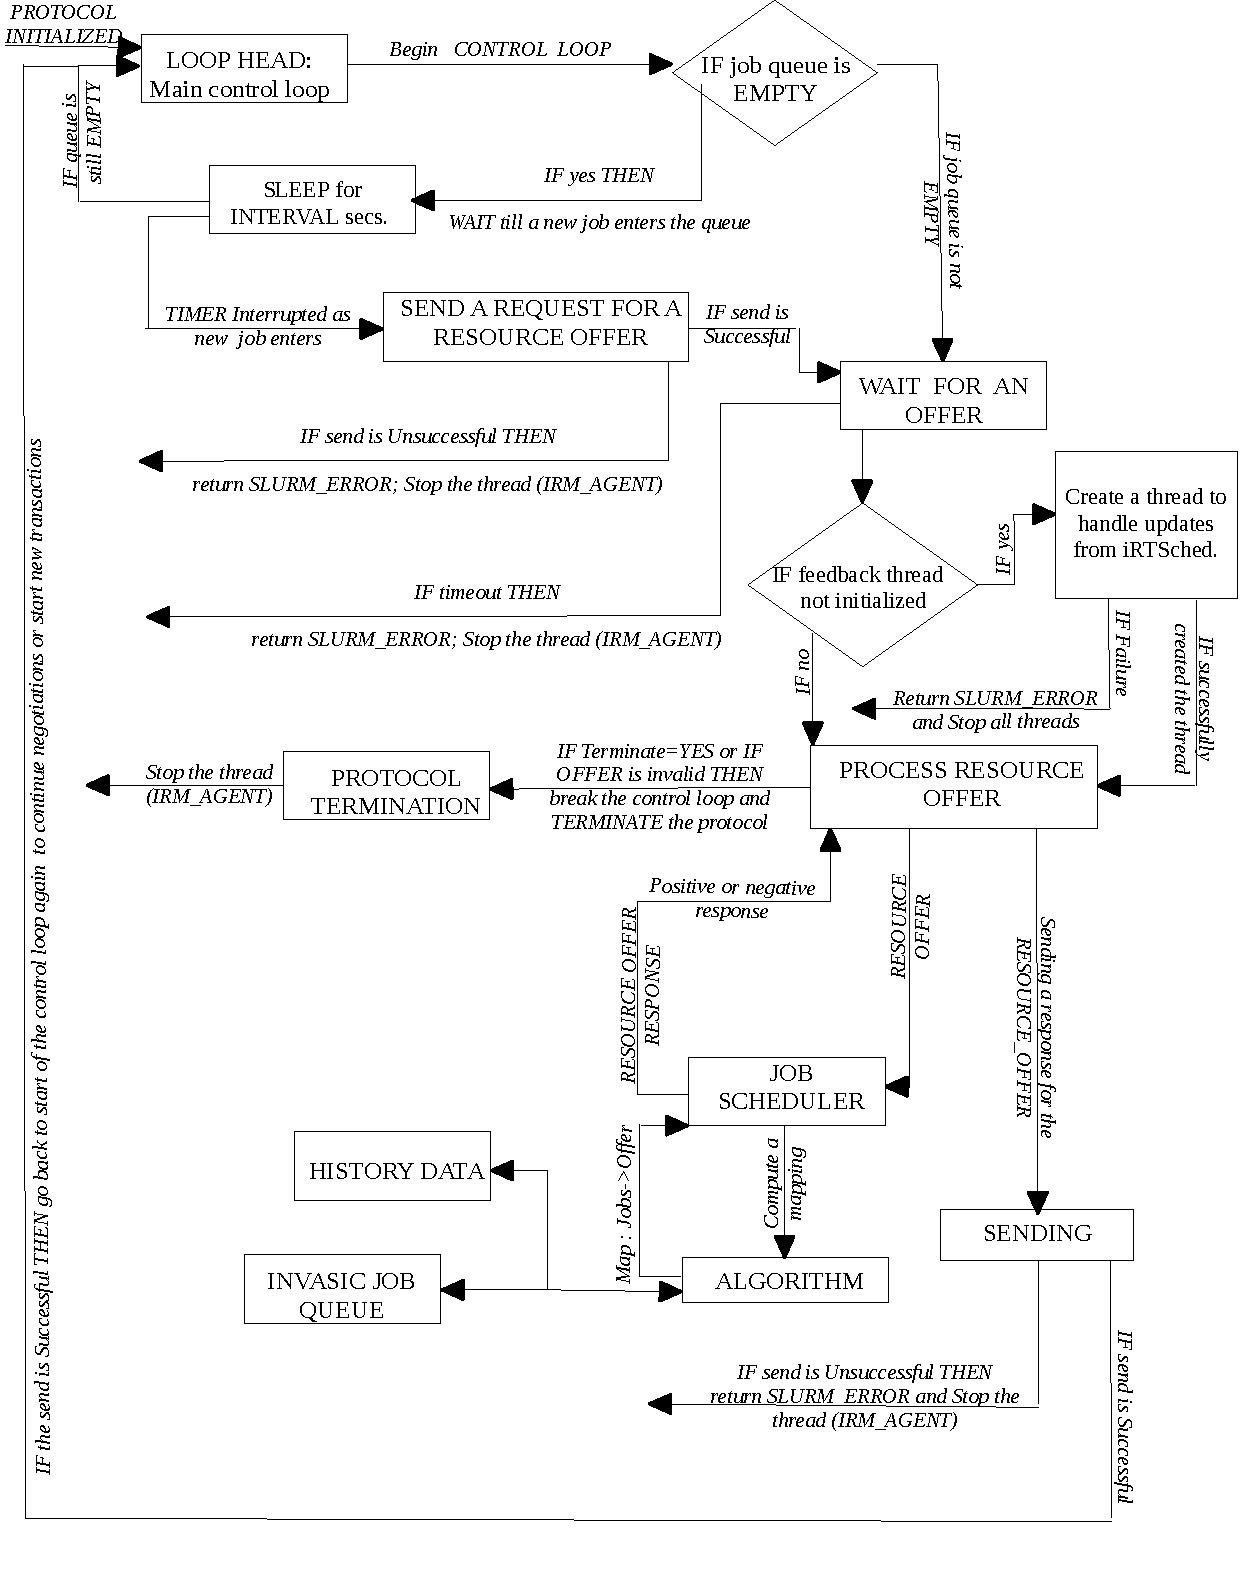
\includegraphics[width=1.0\textwidth, height=210mm]{./figures/iBSched.pdf}
%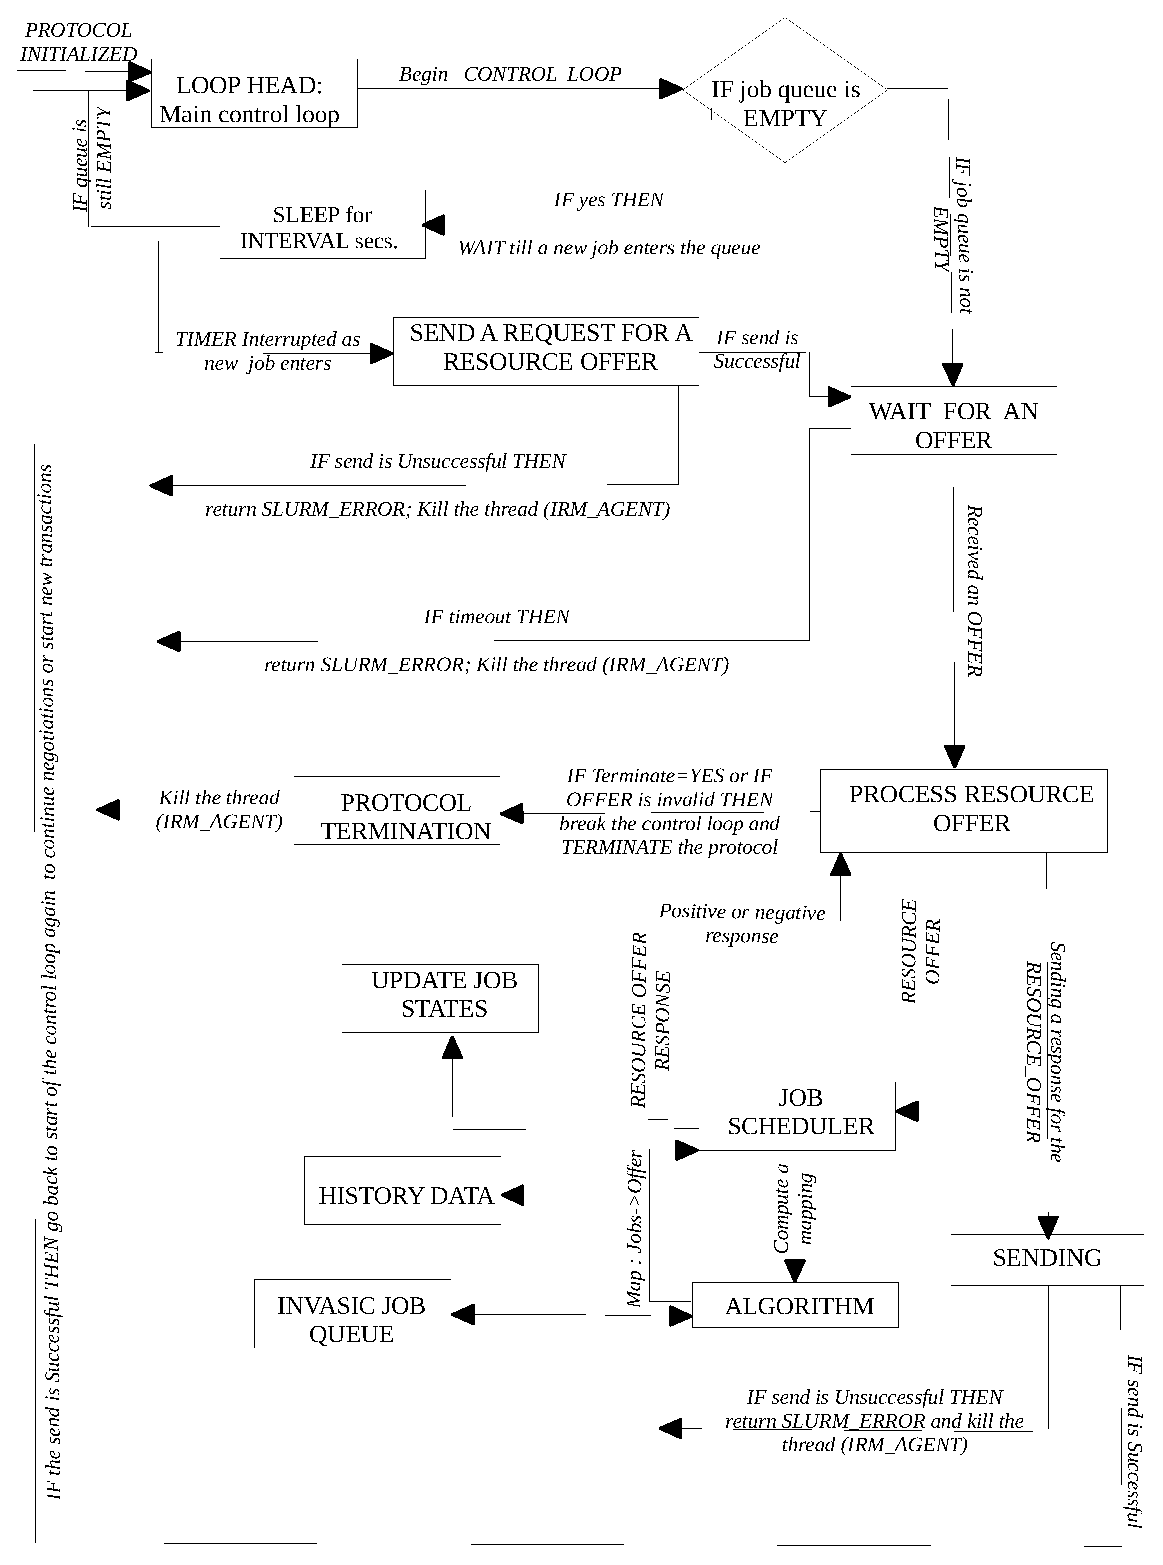
\includegraphics[width=1.0\textwidth, height=180mm]{./figures/Negotiation.eps}
\caption{iBSched}
\label{fig:Neg}
\end{figure}
\subsection{iRTSched}
\begin{figure}[!htbp]
\centering
%\includegraphics[width=1.0\textwidth, height=180mm]{./figures/iBSched.eps}
%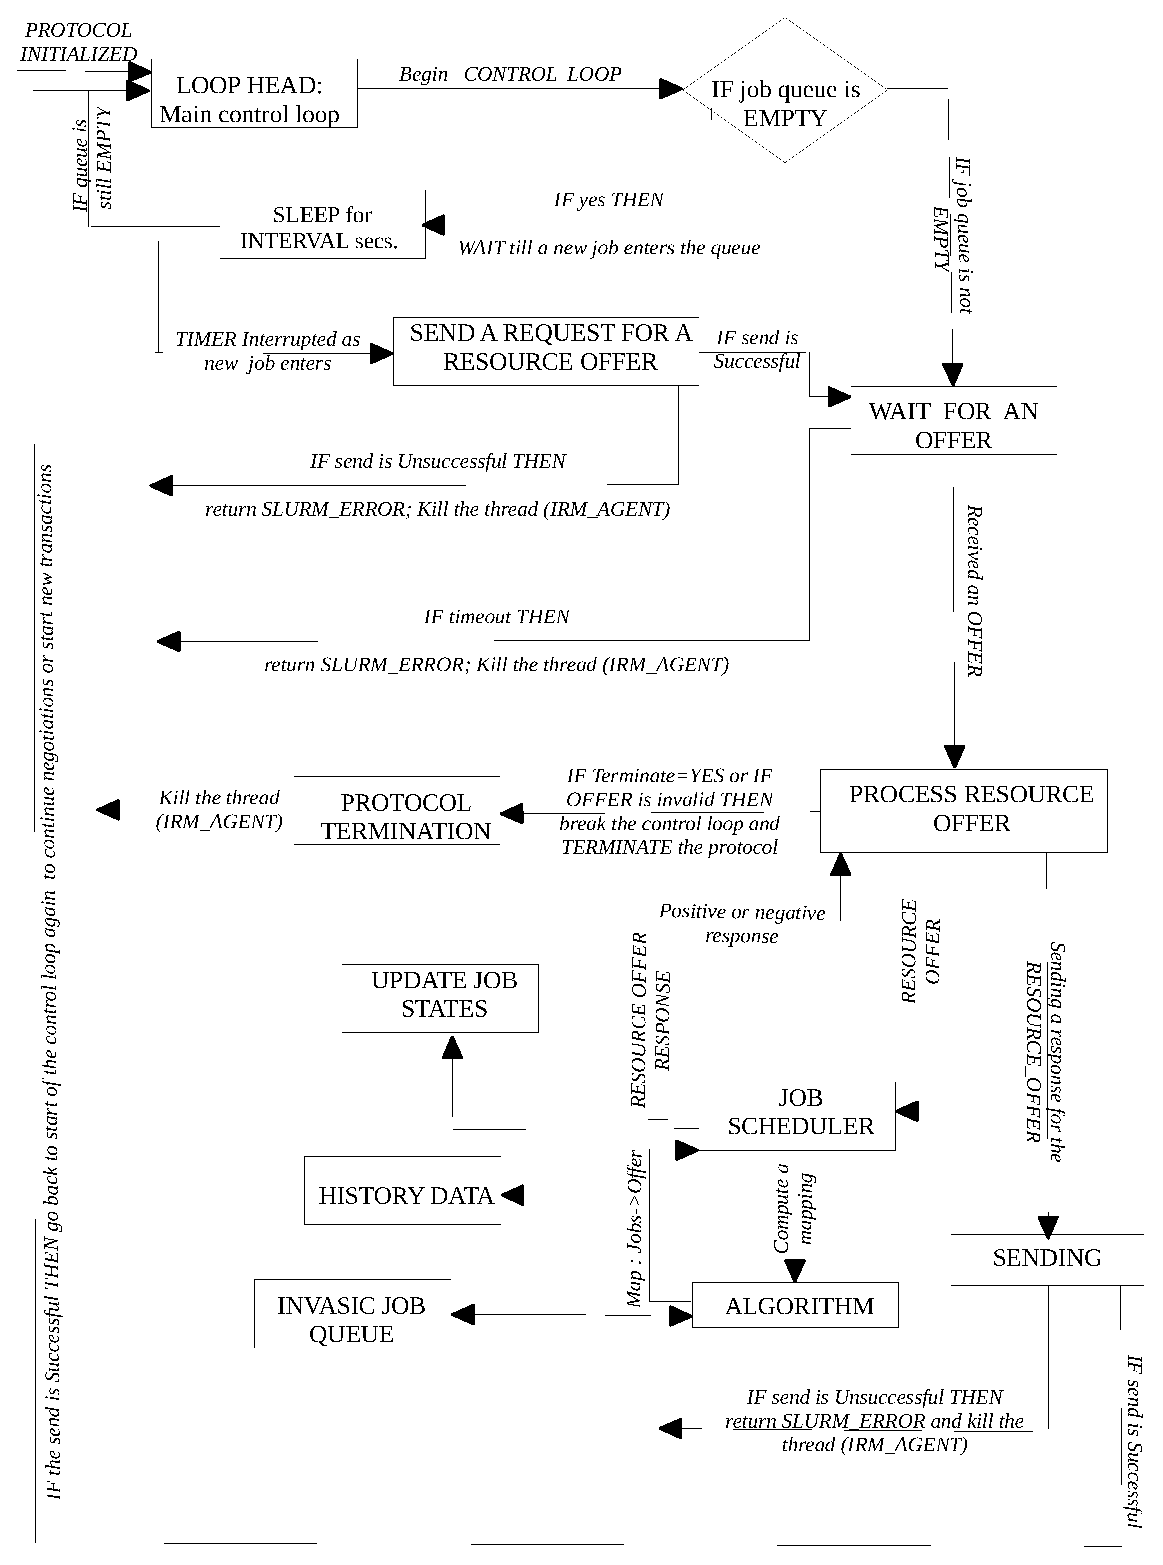
\includegraphics[width=1.0\textwidth, height=180mm]{./figures/Negotiation.eps}
\caption{iRTSched}
\label{fig:Neg}
\end{figure}
